\subsection{Matched filter on enhanced image}
The result of this step is shown in Figure \ref{fig:MatchedResult1}, \ref{fig:MatchedResult2}, \ref{fig:MatchedResult3}.

\begin{figure}
\begin{subfigure}{0.5\textwidth}
    \centering
    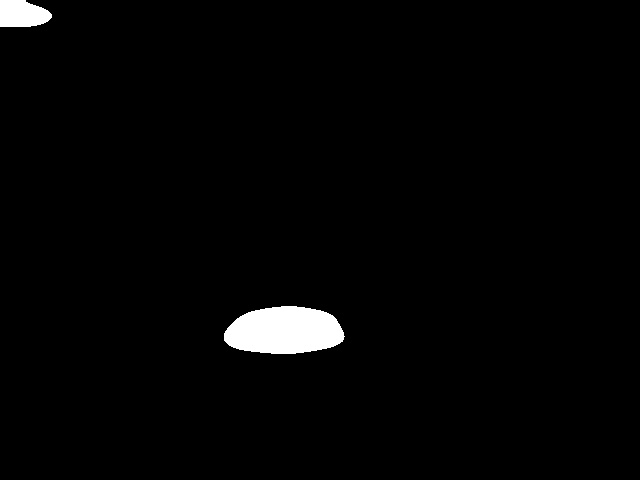
\includegraphics[width=0.9\linewidth]{./img/experiment/stage.6/good}
    \caption{Final result}
\end{subfigure}
\begin{subfigure}{0.5\textwidth}
    \centering
    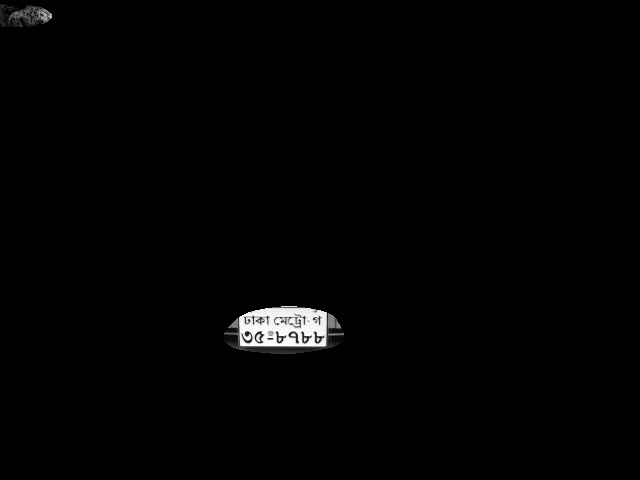
\includegraphics[width=0.9\linewidth]{./img/experiment/stage.6/-3-good}
    \caption{A see-through view with original image}
\end{subfigure}
\caption{After applying matched filter on a good image}
\label{fig:MatchedResult1}
\end{figure}


\begin{figure}
\begin{subfigure}{0.5\textwidth}
    \centering
    
\includegraphics[width=0.9\linewidth]{./img/experiment/stage.6/small}
    \caption{Final result}
\end{subfigure}
\begin{subfigure}{0.5\textwidth}
    \centering
    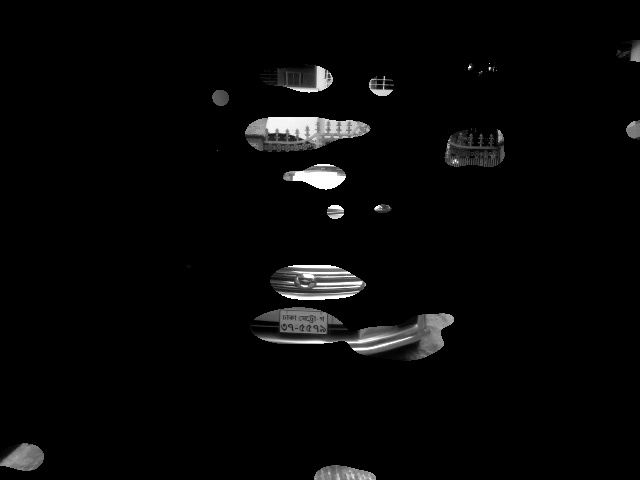
\includegraphics[width=0.9\linewidth]{./img/experiment/stage.6/-3-small}
    \caption{A see-through view with original image}
\end{subfigure}
\caption{After applying matched filter on a small image}
\label{fig:MatchedResult2}
\end{figure}



\begin{figure}
\begin{subfigure}{0.5\textwidth}
    \centering
    
\includegraphics[width=0.9\linewidth]{./img/experiment/stage.6/bumper}
    \caption{Final result}
\end{subfigure}
\begin{subfigure}{0.5\textwidth}
    \centering
    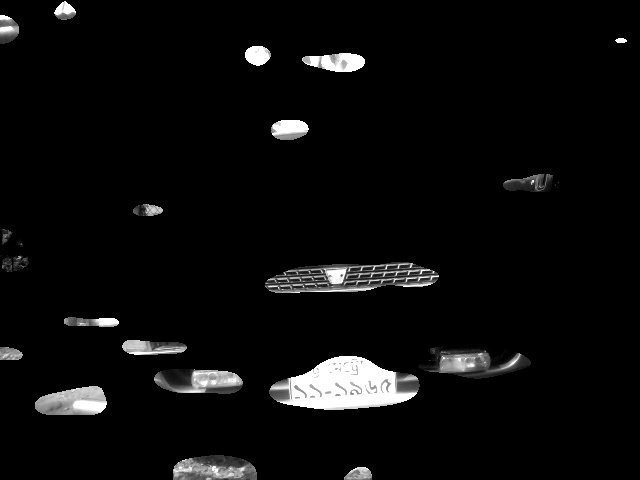
\includegraphics[width=0.9\linewidth]{./img/experiment/stage.6/-3-bumper}
    \caption{A see-through view with original image}
\end{subfigure}
\caption{After applying matched filter on a bright image}
\label{fig:MatchedResult3}
\end{figure}
